\chapter{The Logging Mechanism of Dresden OCL2 for Eclipse}
\label{chapter:logging}

\begin{flushright}
\textit{Chapter written by Claas Wilke}
\end{flushright}

\acl{DOT4Eclipse} uses a \keyword{Log4j Logger} to log method entries, exits and errors during the toolkit's execution. If you run \acl{DOT4Eclipse} as source code plug-ins from an Eclipse workspace, you might receive exceptions like following, although the toolkit works correctly. 

\begin{center}
\reference{log4j:ERROR Could not connect to remote log4j server at [localhost].}
\end{center}

The reason is that the Log4j Logger tries to sent the logged events to a server running at \url{localhost}. To solve this problem (if you want to) you have to install and setup a logging server at your computer. One logging server you might use is called \keyword{Chainsaw} and available at the Apache Logging website \cite{WWW:chainsaw}. If you start Chainsaw, set up a \keyword{SocketReceiver} at port \keyword{4445 (Old Style/Standard Chainsaw Port)} (see figure \ref{pic:logging:chainsaw01}).

\begin{figure}[!htbp]
	\centering
	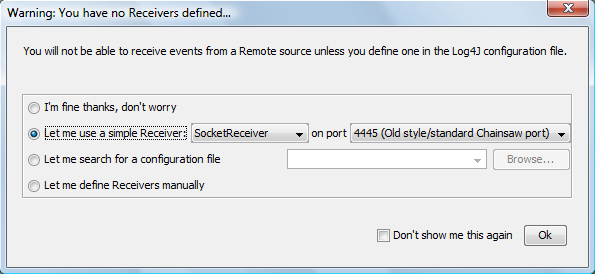
\includegraphics[width=0.8\linewidth]{figures/logging/chainsaw01}
	\caption{Setting up a simple SocketReceiver in Chainsaw.}
	\label{pic:logging:chainsaw01}
\end{figure}